% =============================================================================
%  Sección 3: Sustentabilidad a Largo Plazo: Degradación vs. Remediación
% =============================================================================

\section{Sustentabilidad a Largo Plazo: Degradación vs. Remediación}
En esta sección exploraremos como la resilencia urbana ha favorecido la creación de nuevos ecosistemas biológicos 
y sociales, siendo un reflejo de la identidad de los pobladores y su conciencia sobre el ambiente que los rodea. 
Destacando la intervención de los pobladores, turistas y políticas públicas que (en algunos casos) puede favorecer al 
mantenimiento del ecosistema y su preservación en la identidad de los habitantes circundantes. Recordando que los Humedales 
no solo son un espacio donde florece la vida y la vegetación, también pueden ser motivo de identidad y orgullo.

\subsection{El riesgo de pérdida en Xochimilco}

El sistema lacustre de Xochimilco enfrenta un riesgo crítico de pérdida de funcionalidad debido a la fragmentación del territorio. 
El deterioro ambiental se ha agudizado por la ausencia de red de drenaje y la proliferación de descargas de aguas grises y negras 
directamente a los canales \cite{rojas2020deterioro}. A este escenario se suma la presión por megaproyectos de infraestructura, 
como el puente vehicular en Periférico Sur, el cual amenaza con dividir el humedal y destruir el hábitat de especies endémicas como 
el ajolote (\textit{Ambystoma mexicanum}) \cite{segob2020proposicion}.

Frente a esta degradación, el Gobierno de la CDMX ha intervenido el \textbf{Parque Ecológico de Xochimilco} en la zona de Cuemanco, 
rehabilitando una superficie de 83.65 hectáreas \cite{sedema2022programa}. Esta intervención incluyó el acondicionamiento del Lago Huetzalin y 
el mantenimiento de 1,225 ahuehuetes y ahuejotes, fundamentales para la retención del sustrato chinampero \cite{sedema2022programa}.

Aunque el ajolote se ha consolidad como un animal endémico y símbolo de los humedales de Xochimilco, es importante destacar que el museo del mismo,
\textit{Museo Nacional del Ajolote: "Ajolotitlán"}, no se encuentra en dicho ecosistema, si no en la alcaldía Álvaro Obregón al Poniente de la 
Ciudad de México. Lo que hace una fuerte contradicción en la preservación de la cultura, identidad y patriomonio del humedal.

\subsubsection*{Impacto Social y Cultural: El Escenario de Cuemanco}

La sustentabilidad de este humedal no solo es ecológica, sino profundamente social. El área de Cuemanco funciona como un nodo cultural donde la identidad
 histórica se preserva mediante eventos masivos que atraen el turismo nacional e internacional, como el espectáculo de "La Llorona" \cite{civitatis2024llorona}. 
 Este evento, que combina música, danza y teatro sobre trajineras, utiliza el paisaje natural como escenario vivo, reafirmando el valor del humedal como patrimonio 
 inmaterial \cite{trajineras2024llorona}.

\begin{figure}[H] % Usamos [H] para fijar la posición como se definió en Comands.tex 
    \centering
    % Primera Subfigura
    \begin{subfigure}[b]{0.32\textwidth}
        \centering
        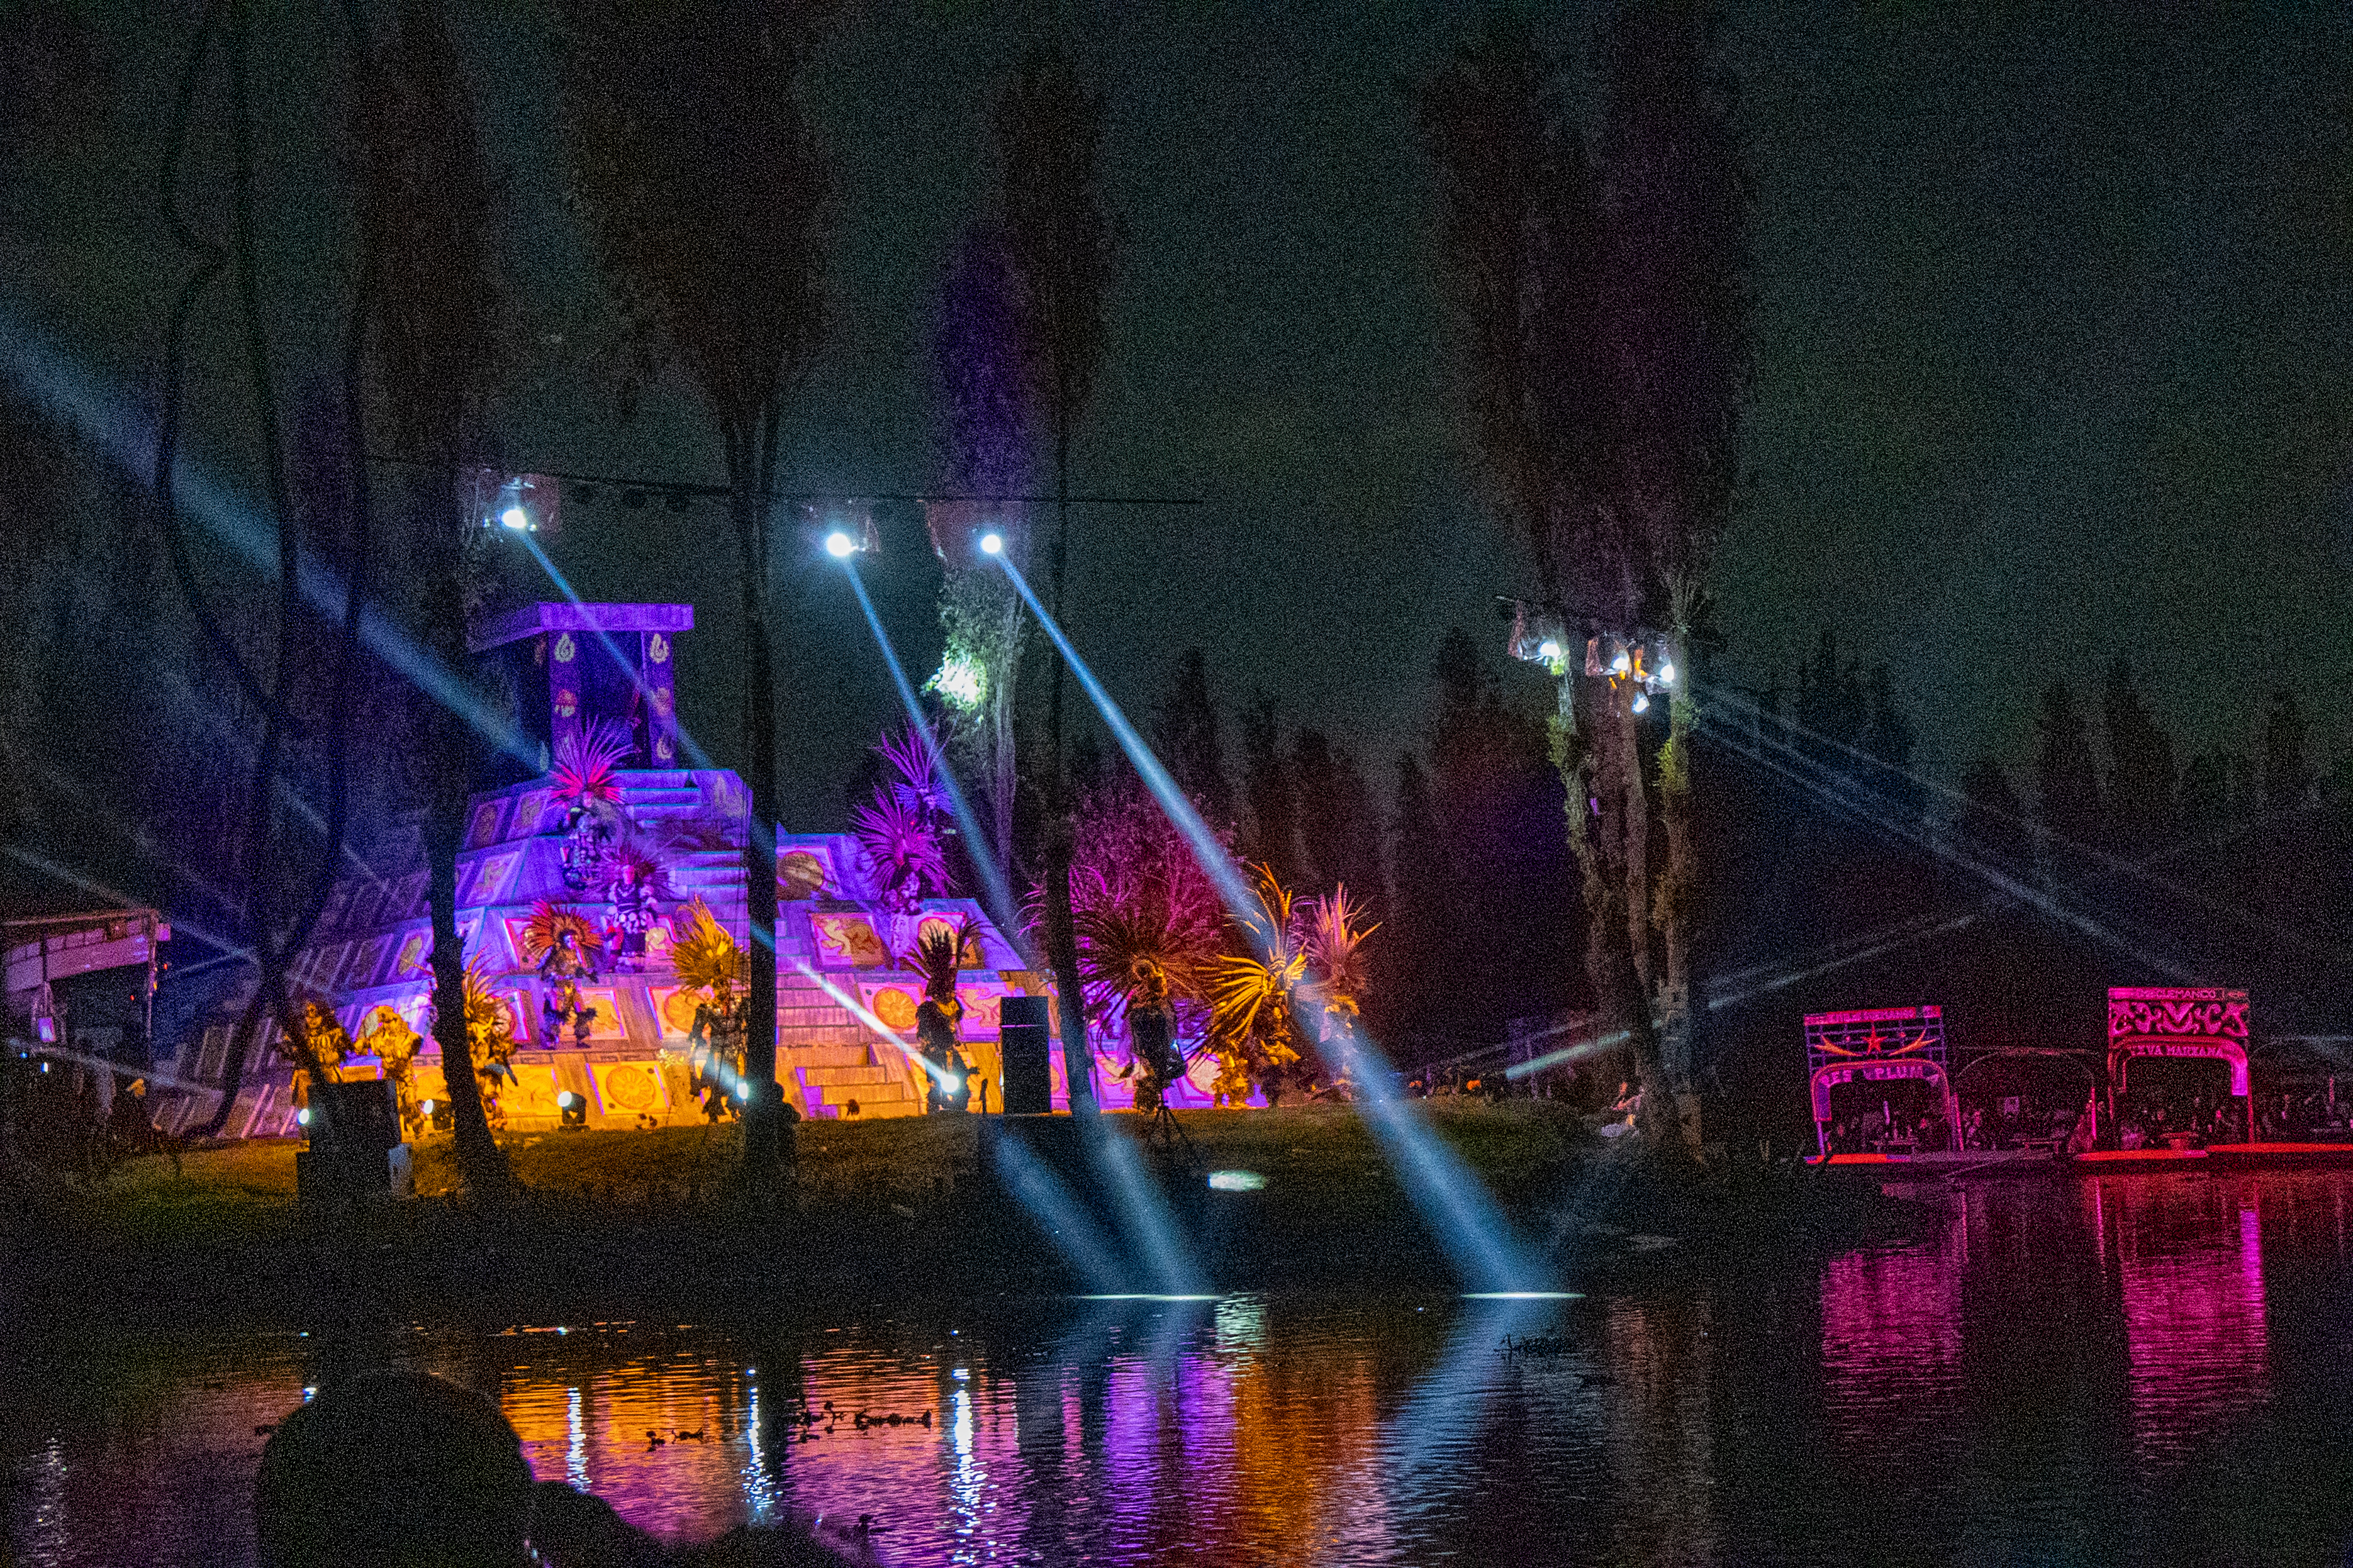
\includegraphics[width=\textwidth]{img/FotoLlorona3.JPEG}
        \caption{Vista del escenario.}
        \label{fig:llorona_escenario}
    \end{subfigure}
    \hfill
    % Segunda Subfigura
    \begin{subfigure}[b]{0.32\textwidth}
        \centering
        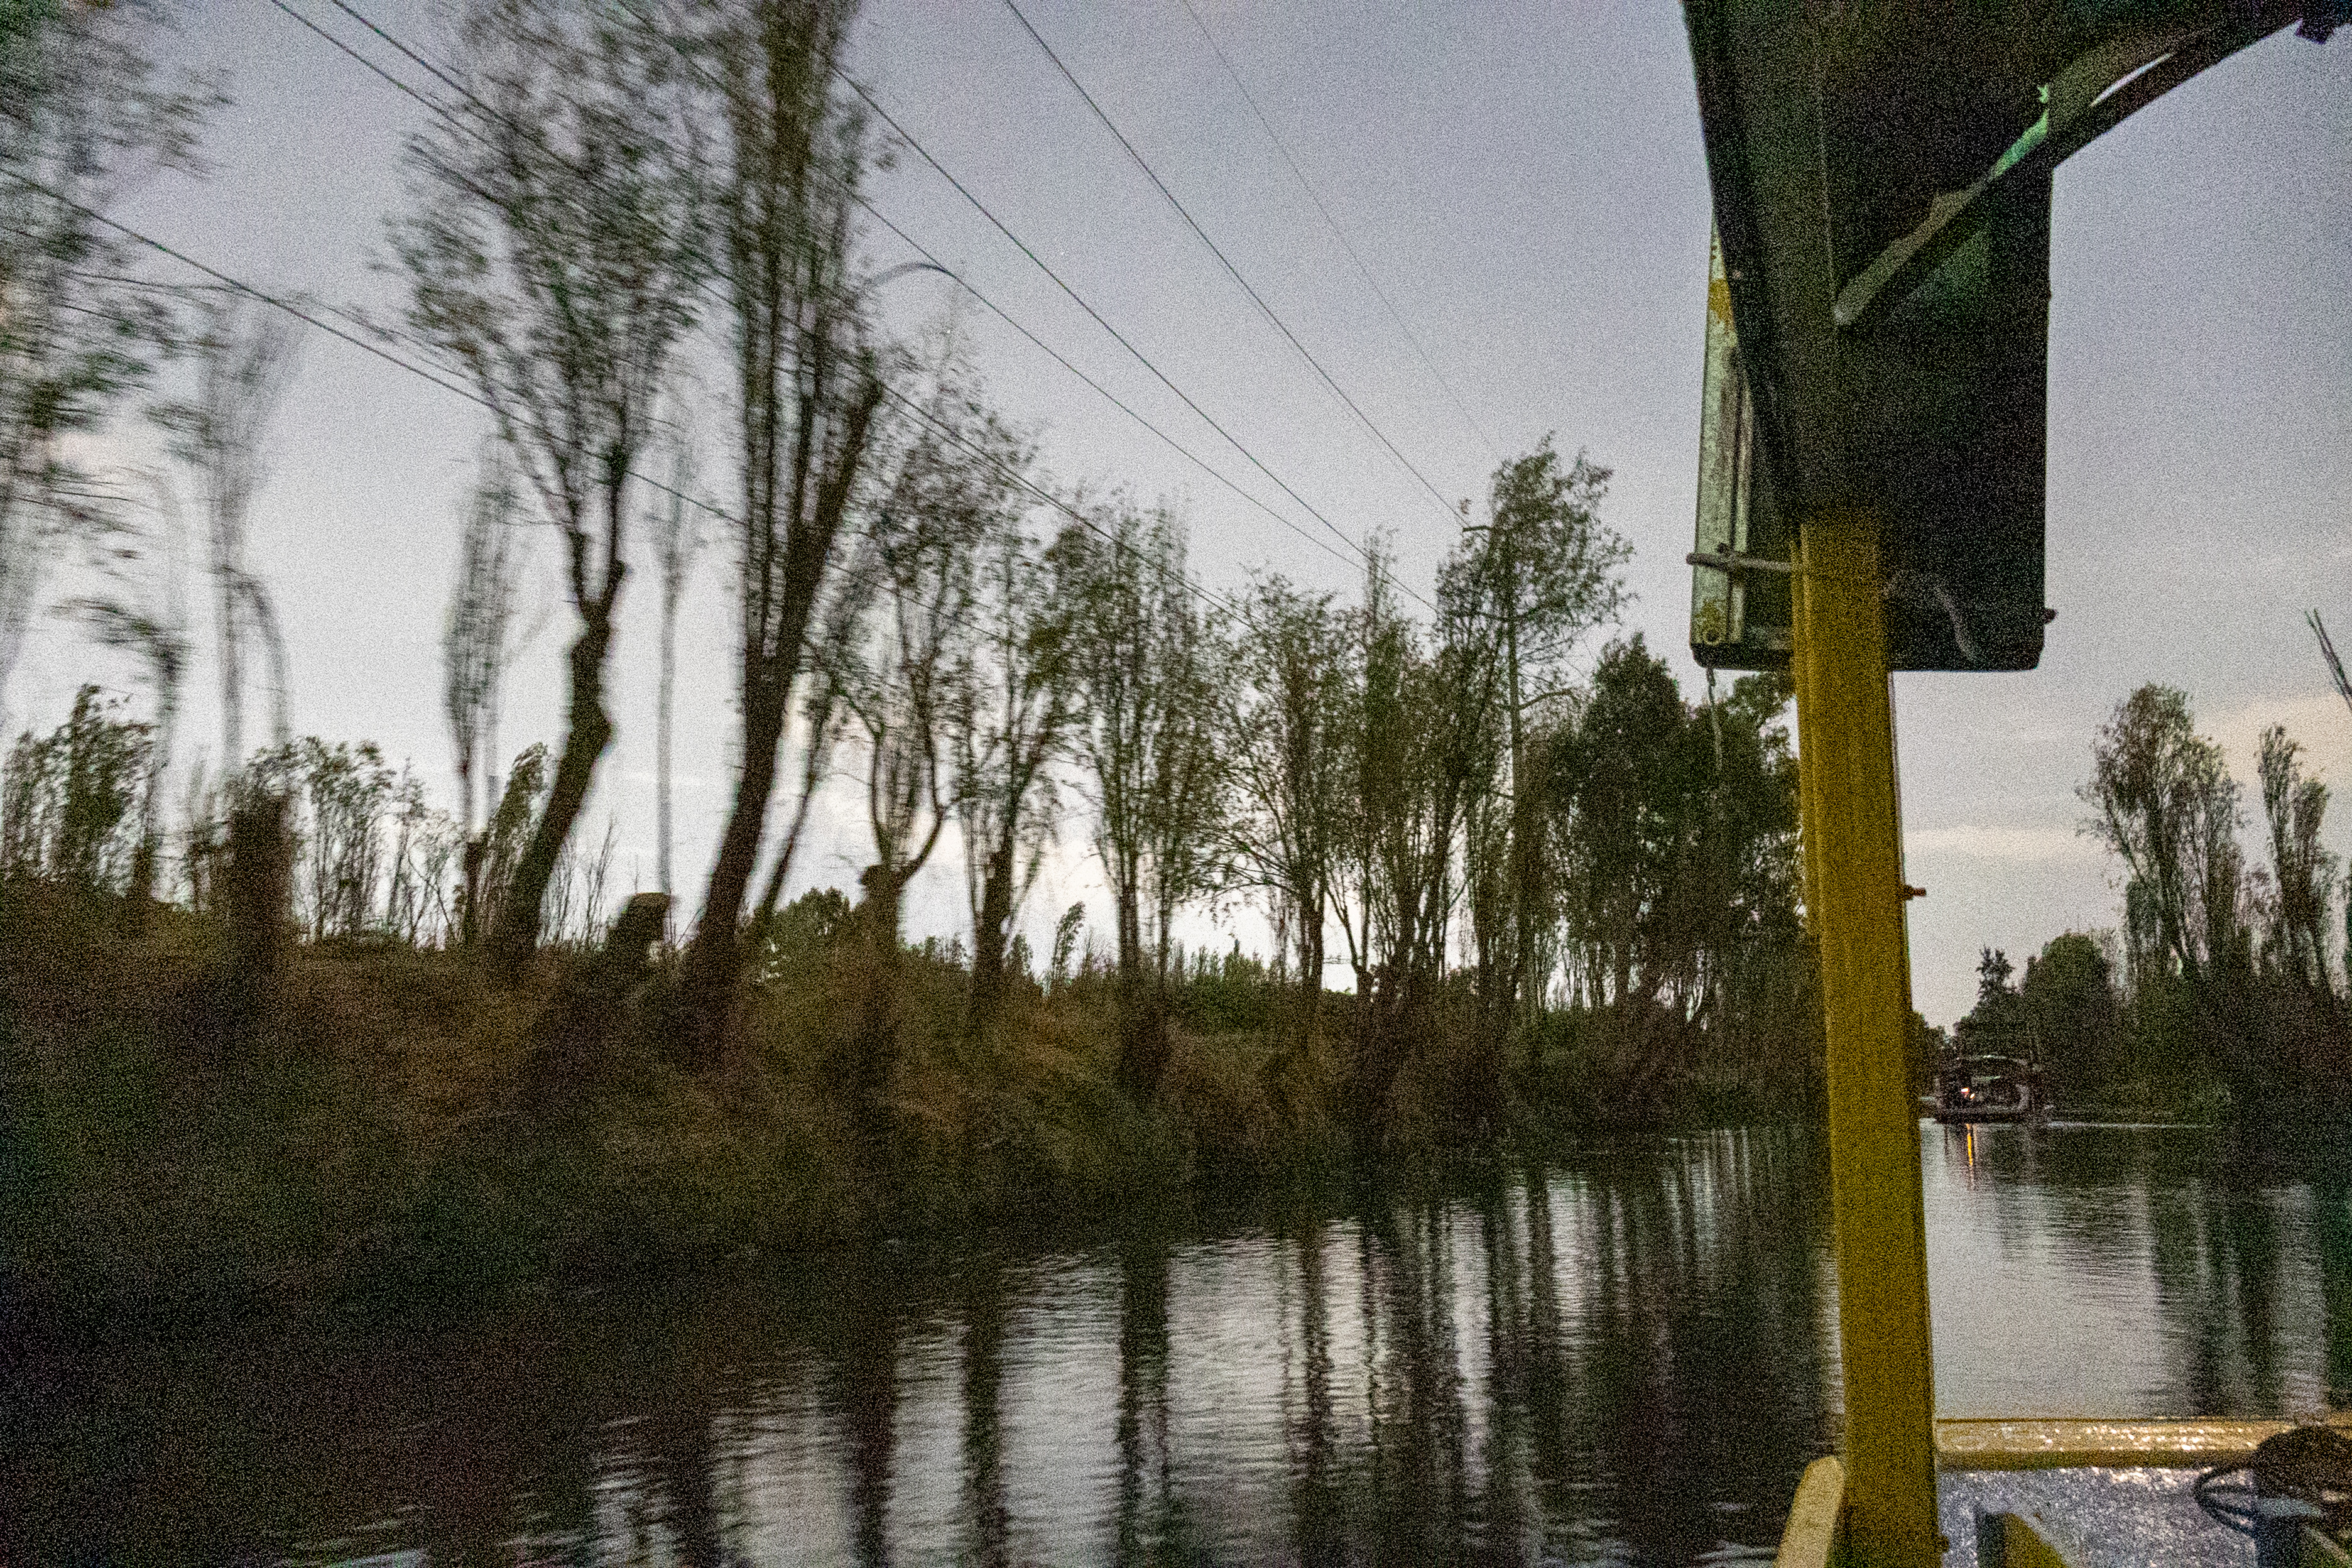
\includegraphics[width=\textwidth]{img/FotoLlorona2.JPEG}
        \caption{Trajineras en Cuemanco.}
        \label{fig:llorona_trajineras}
    \end{subfigure}
    \hfill
    % Tercera Subfigura
    \begin{subfigure}[b]{0.32\textwidth}
        \centering
        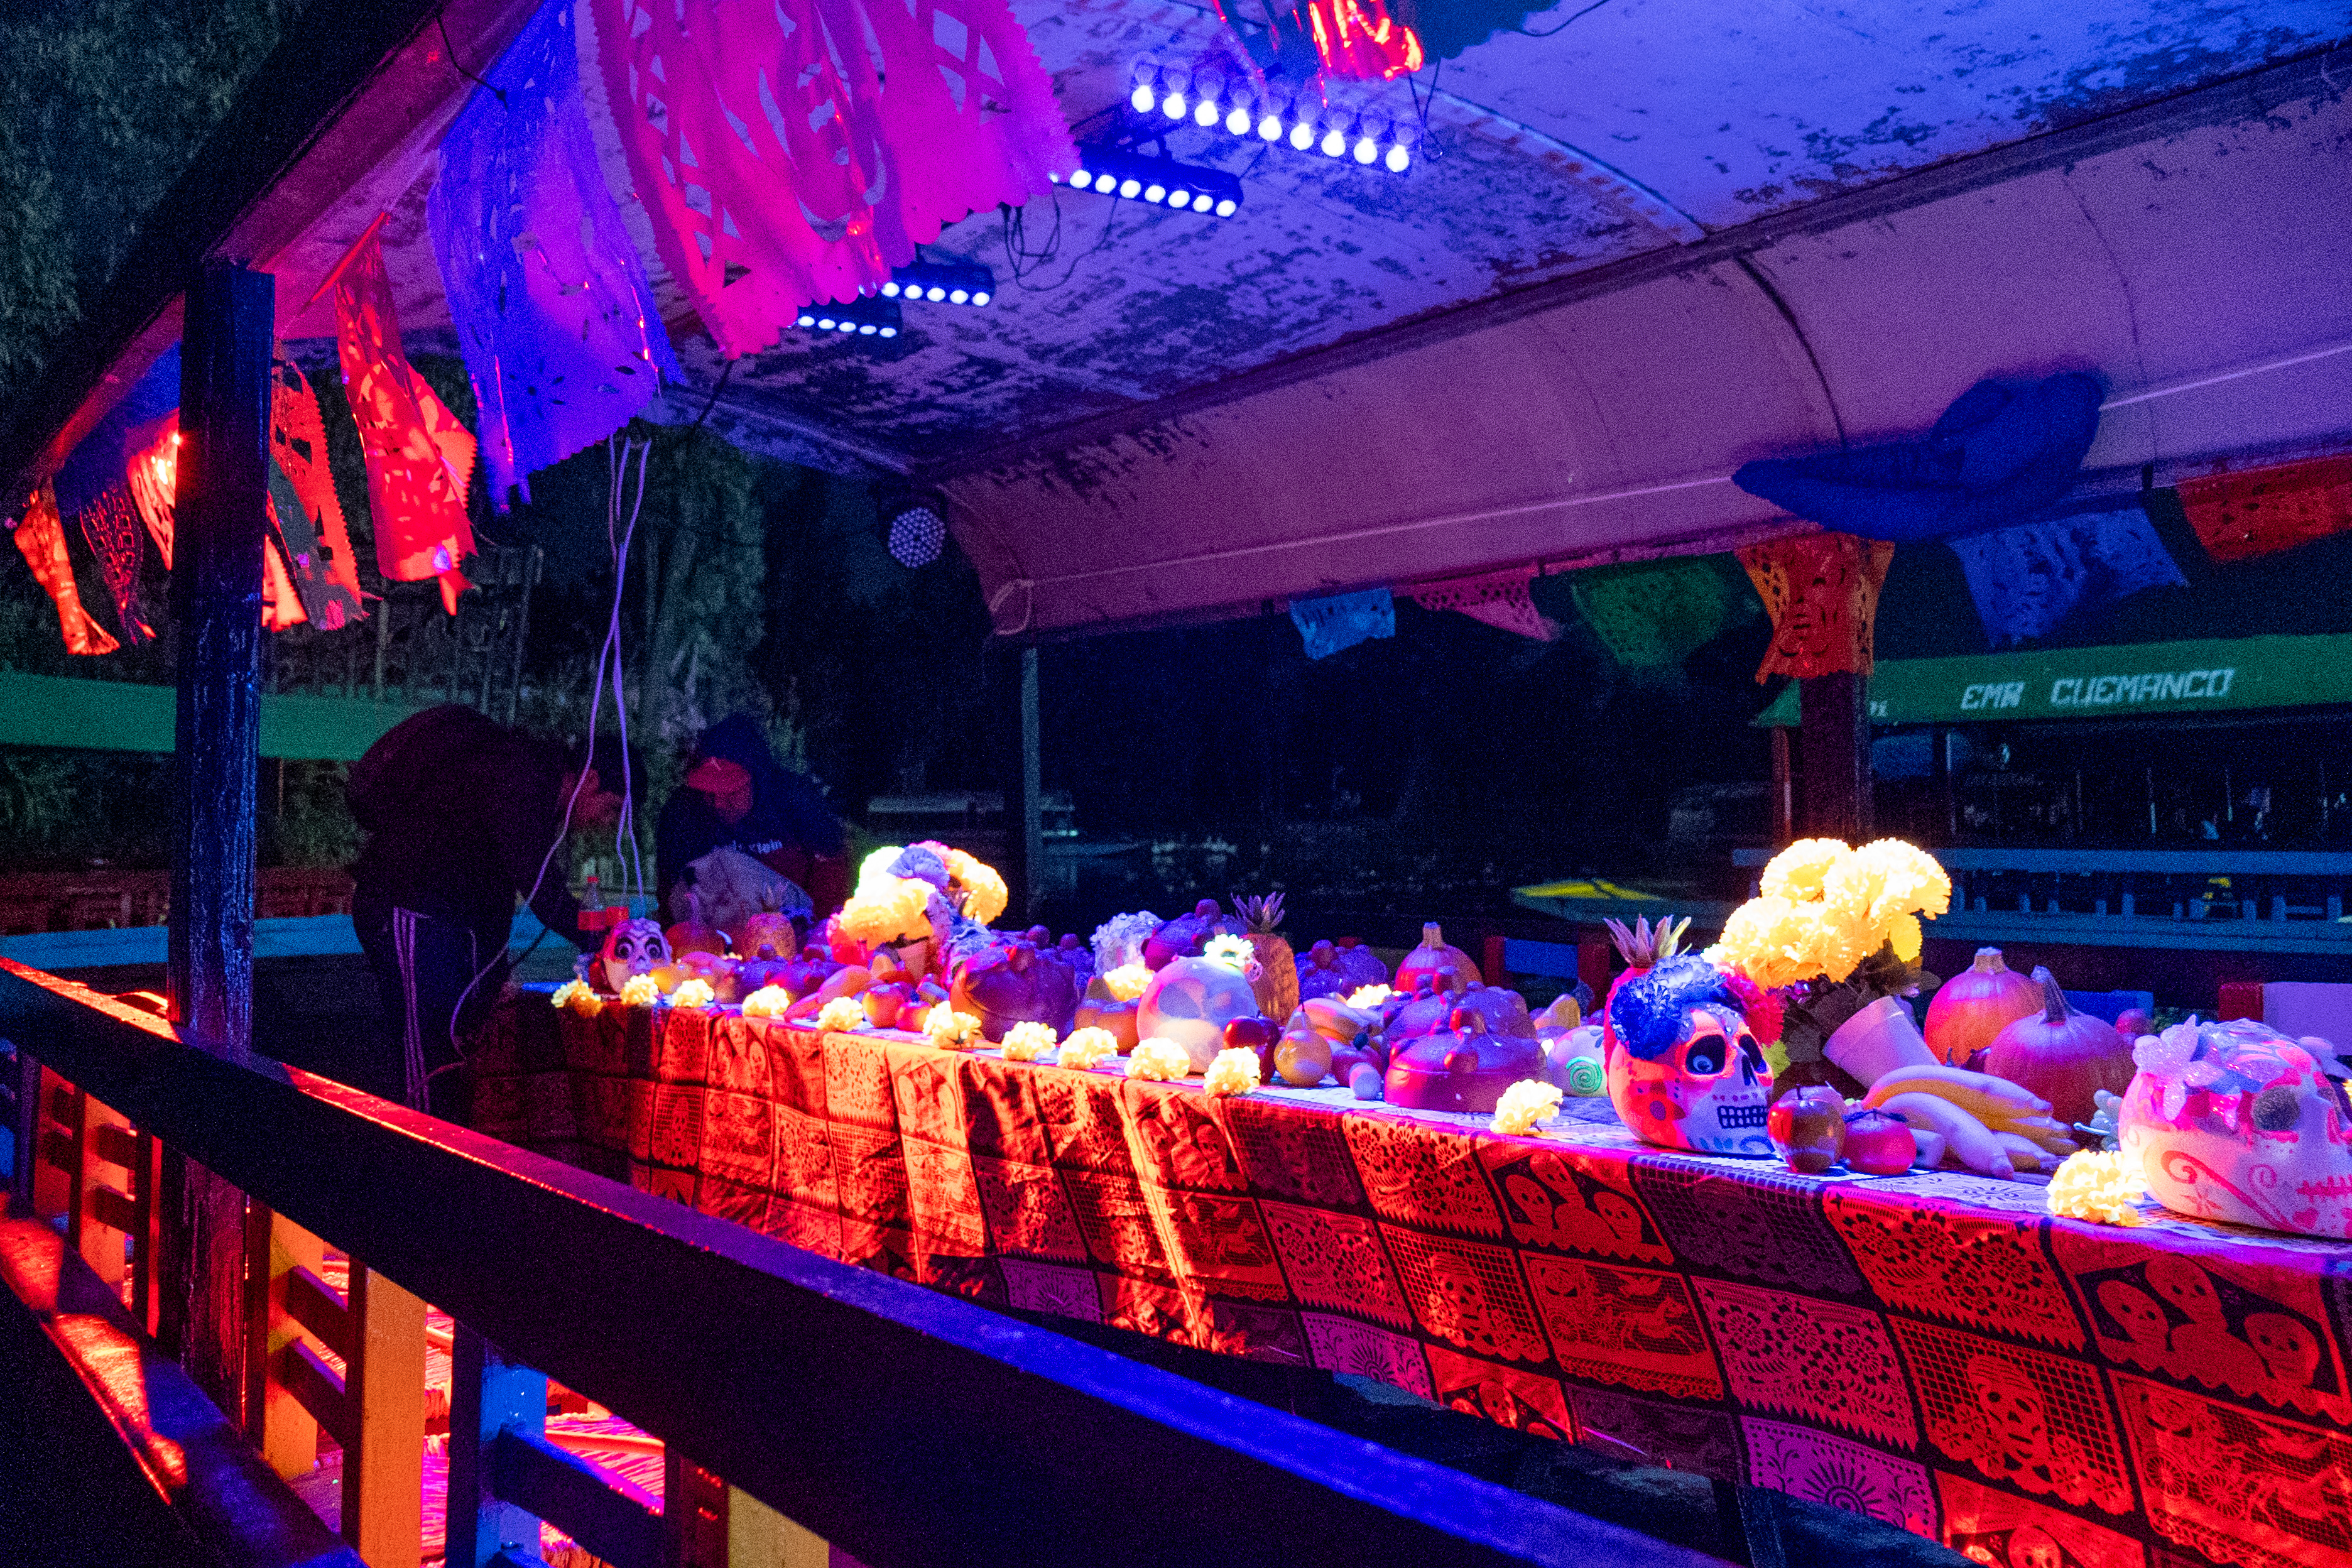
\includegraphics[width=\textwidth]{img/FotoLlorona1.JPEG}
        \caption{Iluminación nocturna.}
        \label{fig:llorona_luces}
    \end{subfigure}

    \vspace{10pt} % Espacio entre imágenes y pie de figura
    \caption{Espectáculo cultural en el humedal de Cuemanco.}
    \fuentefigura{Autoría propia tomada en el año 2025.} % Usando tu comando personalizado 
    \label{fig:espectaculo_llorona}
\end{figure}



\subsection{La ingeniería ecológica en Aragón}
A diferencia de la degradación por ocupación irregular, el \textbf{Bosque de San Juan de Aragón} representa un modelo de remediación activa mediante la ingeniería 
ecológica. El objetivo principal ha sido mejorar la calidad del agua del lago y recuperar la biodiversidad en una zona altamente urbanizada \cite{sedema2022programa}. 
El proyecto contempla la intervención de 57.27 hectáreas y la operación de dos humedales artificiales; el segundo de ellos cuenta con una extensión de 3,100 $m^2$ y 
una capacidad de filtración de 140,000 $m^3$ en 24 horas \cite{sedema2022programa}.

\begin{figure}[ht]
    \centering
    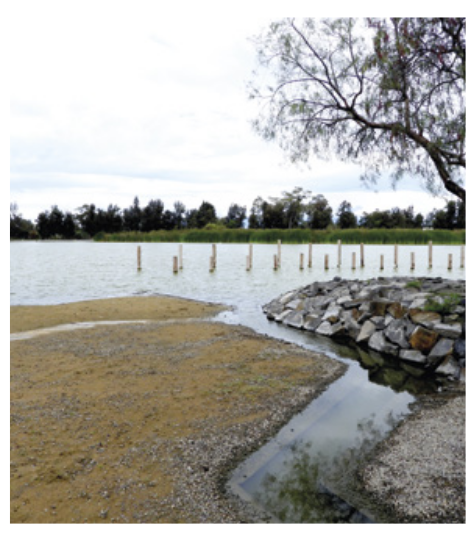
\includegraphics[width=0.8\textwidth]{img/Aragon_vista.png}
    \caption{Vista panorámica del Bosque de San Juan de Aragón y su sistema de humedales artificiales \cite{sedema2022programa}.}
    \label{fig:aragon_vista}
\end{figure}

Esta visión de sustentabilidad destaca por la participación de la comunidad universitaria. Un equipo interdisciplinario de la UNAM ha desarrollado tecnología propia para estos 
sistemas de tratamiento biológico, demostrando que la academia puede generar soluciones basadas en la naturaleza con un alto impacto social al triplicar la cantidad de especies de 
aves en la zona \cite{agua2020aragon, sedema2022programa}. Este modelo valida que la intervención humana, bajo principios científicos, es capaz de sanar entornos urbanos degradados.

